\documentclass{article}

\usepackage{stmaryrd}
\usepackage{amssymb}
\usepackage{tikz}
\usetikzlibrary{positioning}

\title{Interaction Diagram - Delete User}
\author{ Adam Hammes }

% no page number at bottom
\pagenumbering{gobble}

\begin{document}
\maketitle

\begin{center}

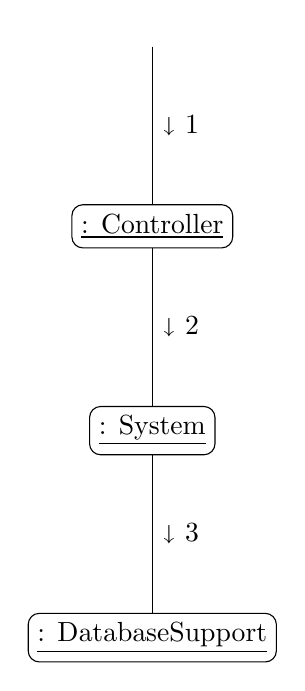
\begin{tikzpicture}[
  auto,
  block/.style = {
    rectangle,
    draw=black,
    align=center,
    rounded corners
  },
  multiple/.style = {
    rectangle, draw, rounded corners, fill= white,
    text width=9em, align= center,
    copy shadow = {
      ,fill=white, draw=black,
      shadow xshift=0.5mm, shadow yshift=-0.5mm
    }
  }
]
\node[] (start)  {};

\node[block, below = 2cm of start] (controller) {\underline{: Controller}};
\node[block, below = 2cm of controller] (system) {\underline{: System}};
\node[block, below = 2 cm of system] (DbSupport) {\underline{: DatabaseSupport}};

\draw (start) -- (controller) node[midway]{$\shortdownarrow$ 1};
\draw (controller) -- (system) node[midway]{$\shortdownarrow$ 2};
\draw (system) -- (DbSupport) node[midway]{$\shortdownarrow$ 3};



\end{tikzpicture}

\vspace{0.5cm}

\begin{enumerate}
    \item \texttt{b:=deleteUser(uid:String):boolean}
    \item \texttt{b:=deleteUser(uid:String):boolean}
    \item \texttt{b:=deleteUser(uid:String):boolean}
\end{enumerate}
\end{center}

\end{document}
